\documentclass{article}
\usepackage{tikz}
\usetikzlibrary{decorations.markings}
\begin{document}

 \begin{figure}[h]
\centering
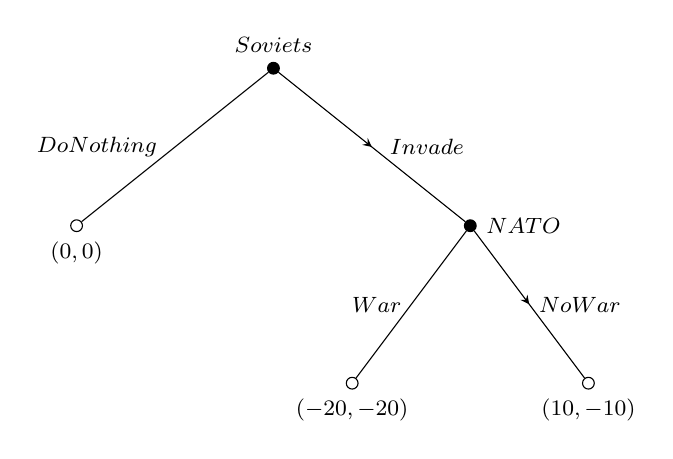
\begin{tikzpicture}[scale=2,font=\footnotesize]
\tikzset{
% Two node styles for game trees: solid and hollow
solid node/.style={circle,draw,inner sep=1.5,fill=black},
hollow node/.style={circle,draw,inner sep=1.5}
}
% Specify spacing for each level of the tree
\tikzstyle{level 1}=[level distance=10mm,sibling distance=25mm]
\tikzstyle{level 2}=[level distance=10mm,sibling distance=15mm]
\tikzstyle arrowstyle=[scale=1]
\tikzstyle directed=[postaction={decorate,decoration={markings,
mark=at position .5 with {\arrow[arrowstyle]{stealth}}}}]
% The Tree
\node(0)[solid node,label=above:{$Soviets$}]{}

child{node(1)[hollow node, label=below:{$(0,0)$}]{}
edge from parent node[left,xshift=-3]{$Do Nothing$}
}
child{node(2)[solid node,label=right:{$NATO$}]{}
child{node[hollow node,label=below:{$(-20,-20)$}]{} edge from parent node[left]{$War$}}
child{node[hollow node,label=below:{$(10,-10)$}]{} edge from parent [directed] node[right]{$No War$}}
edge from parent[directed] node[right,xshift=3]{$Invade$}
};
\end{tikzpicture}
\caption{Soviets--NATO scenario represented in extensive-form game}
\label{fig:NATOUSSR}
\end{figure}


 \begin{figure}[h]
\centering
\begin{tikzpicture}[scale=2,font=\footnotesize]
% Specify spacing for each level of the tree
\tikzstyle{level 1}=[level distance=15mm,sibling distance=25mm]
\tikzstyle{level 2}=[level distance=15mm,sibling distance=15mm]

\tikzset{
% Two node styles for game trees: solid and hollow
solid node/.style={circle,draw,inner sep=1.5,fill=black},
hollow node/.style={circle,draw,inner sep=1.5}
}

% The Tree
\node(0)[solid node,label=above:{$1$}]{}

child{node(1)[solid node,label=right:{$2$}]{}
child{node[hollow node,label=below:{$(2,6)$}]{} edge from parent node[left]{$L'$}}
child{node[hollow node,label=below:{$(0,0)$}]{} edge from parent node[right]{$R'$}}
edge from parent node[left,xshift=-3]{$L$}
}
child{node(2)[solid node,label=right:{$2$}]{}
child{node[hollow node,label=below:{$(3,3)$}]{} edge from parent node[left]{$L'$}}
child{node[hollow node,label=below:{$(0,0)$}]{} edge from parent node[right]{$R'$}}
edge from parent node[right,xshift=3]{$R$}
};

\end{tikzpicture}
\caption{Extensive-form game}
\label{fig:some_extensive_gave}
\end{figure}


\end{document}
